%!Tex Root = ../main.te

% ┌───────┐
% │ Fonts │
% └───────┘
% \newfontfamily\caveat{Caveat}
% \newfontfamily\caveatb{Caveat Brush} % sieht nicht echt genug aus
% \newfontfamily\melissa{Melissa} % mäh
% \newfontfamily\annie{Annie Use Your Telescope} % sieht nicht echt genug aus
% \newfontfamily\cedarville{Cedarville Cursive}
% \newfontfamily\flower{Indie Flower}
% \newfontfamily\kristi{Kristi} % mäh
% \newfontfamily\nanum{NanumPen} % sieht nicht echt genug aus
% \newfontfamily\intolight{Shadows Into Light} % mäh
% \newfontfamily\singleday{Single Day} % mäh

% ┌────────────────┐
% │Handwritten look│
% └────────────────┘
\backgroundsetup{
	scale=1,
	color=black,
	opacity=0.2,
	angle=0,
	position=current page.south west,
	vshift=0mm,
	hshift=0mm,
	contents={
			\begin{tikzpicture}[remember picture,overlay]
				\draw[step=0.25cm] (0,0) grid (\paperwidth,\paperheight);
			\end{tikzpicture}
		}
}

\newcommand{\cul}[2][PrimaryColor]{%
  \setulcolor{#1}% Set the underline color
  \setul{0.1mm}{0.2mm}% Set the underline depth and thickness
  \ul{#2}% Apply the underline with the specified color
}

\newcommand{\nul}[1]{%
  \setulcolor{black}% Set the underline color
  \setul{0.1mm}{0.1mm}% Set the underline depth and thickness
  \ul{#1}% Apply the underline with the specified color
}

% \tikzset{my grid/.style={
%     draw=gray!50,
%     step=1cm,
%     very thin
% }}
%
% % Define a command to draw the grid on every page
% \newcommand{\drawgrid}{
%     \begin{tikzpicture}[overlay, remember picture]
%         \draw[my grid] (current page.south west) grid (current page.north east);
%     \end{tikzpicture}
% }
%
% \pagestyle{fancy}
% \fancyhf{}
% \fancyhead[L]{\drawgrid}

\usetikzlibrary{decorations.pathmorphing}

\tikzset{decoration={random steps,segment length=2mm,amplitude=0.6pt}}

% ┌──────────────────┐
% │ Case distinction │
% └──────────────────┘
% \newtoggle{absolute}
% \toggletrue{absolute}
% \togglefalse{absolute}
% \newcommand{\lpathgraph}[1]{\iftoggle{absolute}{/home/areo/Documents/Studium/Summaries/x/}{./}#1}

% ┌───────┐
% │ Boxes │
% └───────┘
% \DeclareTotalTCBox{\inlinebox}{ s m }
% {verbatim,colback=PrimaryColorDimmed,colframe=PrimaryColor,nobeforeafter,tcbox raise base,top=0mm,bottom=0mm,
%   right=0mm,left=0mm,arc=0.1cm,boxsep=0.1cm}
% {\IfBooleanTF{#1}%
% {\textcolor{PrimaryColor}{\setBold >\enspace\ignorespaces}#2}%
% {#2}}

% \DeclareTotalTCBox{\inlinebox}{ m }
% {standard jigsaw,sharp corners,opacityback=0,colframe=SwitchColor,nobeforeafter,tcbox raise base,boxrule=0.01cm,top=0mm,bottom=0mm,right=0mm,left=0mm,boxsep=0cm}
% % ,arc=0cm
% {#1}
\DeclareTotalTCBox{\inlinebox}{ m }
{enhanced,opacityback=0,colframe=Highlight,nobeforeafter,tcbox raise base,boxrule=0.01cm,top=0mm,bottom=0mm,right=0mm,left=0mm,boxsep=0cm,
	frame style={decorate}
}{#1}

\DeclareTotalTCBox{\key}{ m }
{verbatim,colback=PrimaryColorDimmed,colframe=PrimaryColor,nobeforeafter,tcbox raise base,top=0mm,bottom=0mm,
	right=0mm,left=0mm,arc=0.1cm,boxsep=0.1cm}
{$\mathtt{#1}$}

\newtcolorbox{sidenote}{enhanced,boxrule=0cm,frame hidden,arc=0.2cm,title=Sidenote,attach boxed title to top text left={yshift=-0.2cm},colback=PrimaryColorDimmed,boxed title style={boxrule=0cm,frame hidden,colback=PrimaryColor,arc=0.1cm},fonttitle=\bfseries,
	after title={\hspace{0.2cm}\includegraphics[height=3mm]{./figures/lupe.png}}
}
% drop fuzzy shadow,

\newtcblisting{terminal}{
	enhanced,box align=top,colframe=PrimaryColor,colback=PrimaryColorDimmed,hbox,arc=0.2cm,bottom=0.1cm,top=0.1cm,left=0.1cm,right=0.1cm,boxrule=0.05cm,listing only,minted language=text,listing engine=minted,minted options={escapeinside=||,autogobble}
}

% https://tex.stackexchange.com/questions/593218/nested-inline-math-for-new-command-with-argument
\newcommand{\prompt}{\textcolor{PrimaryColor}{\setBold >\;\ignorespaces}}

\DeclareTCBInputListing{\file}{o m}{
	listing file={#2},enhanced,colframe=PrimaryColor,colback=PrimaryColorDimmed,hbox,,fonttitle=\bfseries,halign title=center,arc=0.2cm,bottom=0.2cm,top=0.1cm,left=0.1cm,right=0.1cm,boxrule=0.5mm,listing only,listing engine=minted,#1}

\DeclareTCBListing{dfile}{o}{
	enhanced,colframe=PrimaryColor,colback=PrimaryColorDimmed,hbox,,fonttitle=\bfseries,halign title=center,arc=0.2cm,bottom=0.2cm,top=0.1cm,left=0.1cm,right=0.1cm,boxrule=0.5mm,listing only,listing engine=minted,#1}

\newtcbinputlisting{\numberedcodebox}[2][]{
	listing file={#2}, enhanced, colframe=PrimaryColor,colback=BoxColor,fonttitle=\bfseries\small,#1,listing only,halign title=center,arc=0.2cm,boxrule=0.05cm,bottom=0.1cm,top=0.1cm,left=0.5cm,right=0.1cm,listing engine=minted,overlay={\begin{tcbclipinterior}\fill[PrimaryColorDimmed] (frame.south west) rectangle ([xshift=0.5cm]frame.north west);\end{tcbclipinterior}}
}

\newtcblisting{dnumberedcodebox}[1][]{
	standard jigsaw, opacityback=0, #1,listing only,boxrule=0cm,bottom=0.1cm,top=0.1cm,left=0.1cm,right=0.1cm,listing engine=minted
}
% \renewcommand{\theFancyVerbLine}{\sffamily
% 	\textcolor{white}{\tiny
% \oldstylenums{\arabic{FancyVerbLine}}}}

% \newtcblisting{dnumberedcodebox}[1][]{
% 	enhanced, colframe=PrimaryColor,colback=BoxColor,fonttitle=\bfseries\tiny,#1,listing only,halign title=center,arc=0.2cm,boxrule=0.05cm,bottom=0.1cm,top=0.1cm,left=0.5cm,right=0.1cm,listing engine=minted,overlay={\begin{tcbclipinterior}\fill[PrimaryColor] (frame.south west) rectangle ([xshift=0.5cm]frame.north west);\end{tcbclipinterior}}
% }

% ┌───────┐
% │ Paths │
% └───────┘
% \newcommand{\script}[2]{\href{openpdf:/home/areo/Documents/Studium/Semester_1_Master/Hardware_Security_and_Trust/slides/Slides annotated/Hardware_Security_and_Trust_all_in_one.pdf:#1}{\inlinebox{#2}}}
\newcommand{\script}[2]{\href{openpdf:/home/areo/Documents/Studium/Semester_2_Master/Concurrency/slides/Concurrency_all_in_one.pdf:#1}{\inlinebox{#2}}}
\newcommand{\lecturenotes}[1]{\href{opentext:#1}{\inlinebox{Lecture Notes}}}
\newcommand{\exercisenotes}[1]{\href{opentext:#1}{\inlinebox{Exercise Notes}}}
\newcommand{\additionalslides}[1]{\href{openpdf:#1:1}{\inlinebox{Additional Slides}}}
\newcommand{\solution}[2]{\href{opentext:#1}{\inlinebox{Solution #2}}}

% /home/areo/Documents/Studium/Semester_2_Master/Concurrency/exercises/lec-01-exercises/01a.MutexWithBuffer.go
% /home/areo/Documents/Studium/Semester_2_Master/Concurrency/exercises/lec-01-exercises/01b.MutexWithoutBuffer.go
% /home/areo/Documents/Studium/Semester_2_Master/Concurrency/exercises/lec-01-exercises/02a.MVarWithBuffer.go
% /home/areo/Documents/Studium/Semester_2_Master/Concurrency/exercises/lec-01-exercises/02b.MVarWithoutBufferNoAnswers.go
% /home/areo/Documents/Studium/Semester_2_Master/Concurrency/exercises/lec-01-exercises/02c.MVarWithoutBuffer.go
